% !TEX root = ../../../main.tex
% 来源：中学数学实验教材·第二册（几何）
% 章节：实验几何 / 基本作图
% 原始文件：1.tex，行 3553-3576
% 类型：tikz
% ---
\begin{tikzpicture}[scale=.8]
\begin{scope}
\tkzDefPoints{0/0/A, 5/0/B, 3/0/C}
\tkzDrawSegments[|-|](A,B)
\tkzLabelSegment[above](A,C){$b$}
\tkzLabelSegment[above](B,C){$c$}
\tkzLabelSegment[below](A,B){$a$}
\tkzCompass[color=black](A,C)
\tkzCompass[color=black](B,C)

\end{scope}
\begin{scope}[xshift=7cm]
	\tkzDefPoints{0/0/A, 5/0/B, 3/1/C}
\tkzDefPoint(30:2){D}


\tkzDrawSegments(A,B A,D B,C)
\tkzLabelSegment[below](A,B){$a$}
\tkzLabelSegment[above](B,C){$c$}
\tkzLabelSegment[above](A,D){$b$}
\tkzCompass[color=black, delta=35](A,D)
\tkzCompass[color=black, delta=35](B,C)
\end{scope}
\end{tikzpicture}
